\documentclass{beamer}
%
% Choose how your presentation looks.
%
% For more themes, color themes and font themes, see:
% http://deic.uab.es/~iblanes/beamer_gallery/index_by_theme.html
%
\mode<presentation>
{
  \usetheme{NYU}      % or try Darmstadt, Madrid, Warsaw, ...
  \usecolortheme{default} % or try albatross, beaver, crane, ...
  \usefonttheme{default}  % or try serif, structurebold, ...
  \setbeamertemplate{navigation symbols}{}
  \setbeamertemplate{caption}[numbered]
} 
\usepackage{listings} 
\usepackage{bera} 

\usepackage[ruled]{algorithm2e}

\usepackage{dsfont}

\usepackage{MnSymbol}%
\usepackage{wasysym}%

\usepackage{booktabs} 

\usepackage[english]{babel}
\usepackage[utf8x]{inputenc}

\title[From Bound Majorization to Stochastic Bound Majorization]{From Bound Majorization to Stochastic Bound Majorization}
\author{Yunian Pan}
\institute{ECE department}
\date{May. 7th 2019}
\titlegraphic{\hfill
\includegraphics[height=1.5cm]{nyu_stacked_color}}

\begin{document}

\begin{frame}{AD machine learning Project}
  \titlepage
\end{frame}

% Uncomment these lines for an automatically generated outline.
%\begin{frame}{Outline}
%  \tableofcontents
%\end{frame}

\section{Outline}

\begin{frame}{From Bound Majorization to Stochastic Bound Majorization}

\begin{itemize}
  \item Theoretical development
  \item Convergence Guarantee
  \item Evaluations
  \item Conclusion
\end{itemize}

\vskip 1cm

\begin{block}{}
  Outperforming state-of-the-art first- and second-order
  optimization methods on various learning tasks
 \end{block}

\end{frame}

\section{Theoretical development}


\begin{frame}{}

For a given i.i.d. dataset $\{(x_1, y_1), \ldots, (x_t, y_t)\}$, $y\in \Omega $ where $|\Omega| = K$, 
setting linear predictors for every data point:
  \begin{equation}
    \begin{aligned}
     &\ln \Pr(y_i | y_i = 1, x_i) = \theta_{1}^{\top } \cdot x_i - \ln Z  \nonumber \\
     &\ln \Pr(y_i | y_i = 2, x_i) = \theta_{2}^{\top } \cdot x_i - \ln Z  \nonumber \\
     &\ldots \ldots \ldots  \\ 
     &\ln \Pr(y_i | y_i = K, x_i) = \theta_{K}^{\top } \cdot x_i - \ln Z  \nonumber \\
    \end{aligned}
   \end{equation}
 \pause \visible<2->{ 
   \begin{block}{}
     normalizer $Z$, prior $\Pr(y = k) = h(y)$, score $\theta_k^{\top} x_i \to \theta^{\top} \textbf{f}_{x_i}(y)$
     Resulting soft-max partition function:
    \begin{equation}
      Z_{x_i}(\theta ) = \sum_{y \in \Omega} h(y) \exp(\theta^{\top} \textbf{f}_{x_i}(y)) 
    \end{equation}
   \end{block}}
  
\end{frame}

\begin{frame}
\begin{block}{Upper bound of Partition}
  Notation setting:
 \begin{enumerate}
  \item $\pi(\cdot): \Omega \to \{1,\ldots,n\} $ s.t. $h(y) = h(\pi^{-1}(j)) = h_j$ and $\textbf{f}(y) = \textbf{f}(\pi^{-1}(j)) = \textbf{f}_j$
  \item $\lambda = \theta - \tilde{\theta}$ 
  \item $Z(\theta) = \sum_{j=1}^{n} \alpha_j \exp(\lambda^{\top}\textbf{f}_j)$, where $\alpha_j = h(j) \exp(\tilde{\theta}^{\top}\textbf{f}_j)$.
 \end{enumerate}
\end{block}
\pause
\visible<2->{\begin{block}{}
  In order to construct the monotonicity we denote $Z_i(\theta) = \sum_{j=1}^{i}\alpha_j \exp(\lambda^{\top}\textbf{f}_j)$, and a trivial bound holds for $i=0$:

  \begin{equation}
    \begin{aligned}
      Z_{0}(\theta ) = 0 \leq z_0 \exp(\frac{1}{2} {\bf\lambda}^{\top} \Sigma_0 \lambda + \lambda^{\top} {\bf\mu}_0)  \nonumber
    \end{aligned}
  \end{equation}
  Where $z_0 = 0^{+},\ \mu_0 = \textbf{0},\ \Sigma_0 = z\bf{I}$.
\end{block}}
\end{frame}


\begin{frame}{Construct bound}
  \begin{block}{}
    As we add another term $\alpha_1 \exp(\lambda^{\top} \bf{f}_1)$, on both side of the above inequality, the bound still holds, 
 \begin{equation}
  \begin{aligned}
   Z_{1}(\theta ) \leq z_0 \exp(\frac{1}{2} \lambda^{\top} \Sigma_0 \lambda + \lambda^{\top} \mu_0) + \alpha_1 \exp(\lambda^{\top}\bf{f}_1)  \nonumber
  \end{aligned}
 \end{equation} 
 \end{block}
 \pause
%The question is that can we 
\visible<2->{Goal: Transform the RHS into quadratic form.
\begin{equation}
  \begin{aligned}
   Z_{1}(\theta )  \leq z_1 \exp(\frac{1}{2} \lambda^{\top} \Sigma_1 \lambda + \lambda^{\top} \mu_1)  \nonumber \label{goal}
  \end{aligned}
 \end{equation} }
 \pause
 %How can we do that 
 \visible<3->{Same recurssive procedure for $Z_{2}(\theta), \ldots, Z_{n}(\theta)$.}
\end{frame}



\begin{frame}{Algebra Work}
Logarithmic transformation:
  \begin{equation}
    \begin{aligned}
     \log Z_{1}(\theta ) &\leq \log z_0 + \log (\exp(\frac{1}{2} \lambda^{\top} \Sigma_0 \lambda + \lambda^{\top} \mu_0) + \frac{\alpha_1}{z_0} \exp(\lambda^{\top}\textbf{f}_1)) \nonumber \\
      & = \log z_0 + \log (\exp(\frac{1}{2} \lambda^{\top} \Sigma_0 \lambda + \lambda^{\top} (\mu_0 - \textbf{f}_1)) + \frac{\alpha_1}{z_0} ) + \lambda^{\top}\textbf{f}_1  \nonumber \\
     \label{inequality3}
    \end{aligned}
   \end{equation}
   \pause
   \visible<2->{
   seperate $\frac{1}{2}w^{\top}w = \frac{1}{2} (\textbf{f}_1 - \mu_0)^{\top} \Sigma_0^{-1} (\textbf{f}_1 - \mu_0)$   
   \begin{equation}
    \begin{aligned}
RHS & = \log z_0 +  \lambda^{\top}\textbf{f}_1 -\frac{1}{2}w^{\top}w + \log\exp \frac{1}{2}w^{\top}w \cdot \exp(\frac{1}{2} \lambda^{\top} \Sigma_0 \lambda + \lambda^{\top} \mu_0) + \frac{\alpha_1}{z_0}) \\
         & = \log z_0 + \lambda^{\top}\textbf{f}_1 -\frac{1}{2}w^{\top}w + \log (\exp(\frac{1}{2} u^{\top} u) + \gamma) \nonumber
    \label{inequality4}
    \end{aligned}
   \end{equation}
   Where $u^{\top} u = \frac{1}{2} (\textbf{f}_1 - \mu_0)^{\top} \Sigma_0^{-1} (\textbf{f}_1 - \mu_0) + \frac{1}{2} \lambda^{\top} \Sigma_0 \lambda + \lambda^{\top} \mu_0$, and $\gamma = \frac{\alpha}{z_0}\exp(\frac{1}{2}w^{\top}w)$
   }
\end{frame}

\begin{frame}{Useful Machinery}
  \begin{lemma}
    For all $u\in R^d$ and $v\in R^d$ and any $\gamma \geq 0$, the bound $\log(\exp(\frac{1}{2}\left\lVert u \right\lVert^2) + \gamma) \leq $
    \begin{equation}
      \log(\exp(\frac{1}{2}\left\lVert v \right\lVert^2) + \gamma) + \frac{ v^{\top} (u- v)}{1 + \gamma \exp(-\frac{1}{2}\left\lVert v \right\lVert^2)} + \frac{1}{2}(u-v)^{\top} (I + \Gamma vv^{\top})(u-v)         \nonumber
    \end{equation}
    holds when the scalar term $\Gamma = \frac{\tanh(\frac{1}{2}\log(\gamma \exp(-\frac{1}{2}\left\lVert v \right\lVert^2))}{2\log(\gamma \exp(-\frac{1}{2}\left\lVert v \right\lVert^2)}$, equality is achieved when $u = v$.
   \label{lemma1}
  \end{lemma}
  \begin{proof}
    see T. Jebara. {\it Multitask sparsity via maximum entropy discrimination. JMLR, 12:75–110,} 2011.
  \end{proof}
\end{frame}


\begin{frame}{Applying Lemma}
%\begin{block}
  \begin{equation}
    \begin{aligned}
     \log Z_1(\theta) & \leq \log z_0 + \lambda^{\top}\textbf{f}_1 - \frac{1}{2} (\textbf{f}_1 - \mu_0)^{\top} \Sigma_0^{-1} (\textbf{f}_1 - \mu_0) \\
            & + \log(\exp(\frac{1}{2}\left\lVert v \right\lVert^2) + \gamma) +  \\ &\frac{ v^{\top} (u- v)}{1 + \gamma \exp(-\frac{1}{2}\left\lVert v \right\lVert^2)} + \frac{1}{2}(u-v)^{\top} (I + \Gamma vv^{\top})(u-v)         \nonumber
         \label{inequality5}
    \end{aligned}
  \end{equation}
Use undetermined coefficients method, recall the goal $\ref{goal}$:

\begin{equation}
  \begin{aligned}
    z_1 &= z_0 + \alpha_1 \\ \nonumber 
    \mu_1 &=  \mu_0 + \frac{\alpha_1}{z_0 + \alpha_1} (\textbf{f}_1 - \mu_0) \\
    \Sigma_1 &= \Sigma_0 + \frac{\tanh(\frac{1}{2}\log(\frac{\alpha_1}{z_0})}{2\log(\frac{\alpha_1}{z_0})} (\textbf{f}_1 - \mu_0)(\textbf{f}_1 - \mu_0)^{\top}
     \end{aligned}
 \end{equation} 


\end{frame}

\begin{frame}{Algorithm1}
  \begin{algorithm}[H]
    \caption{Compute Bound}
    \KwIn{Parameters $\tilde{\theta},\ \textbf{f}(y),\ h(y)$}
    \textbf{Initialize:} $z \leftarrow 0^{+},\ \mu\leftarrow 0,\ \Sigma\leftarrow zI$\;    
    \For{ each $y\in \Omega$}{
      $\alpha = h(y)\exp(\tilde{\theta}^{\top}f(y))$ \\
      $\mu =  \mu + \frac{\alpha}{z+\alpha} (\textbf{f}(y) - \mu)$ \\
      $\Sigma = \Sigma + \frac{\tanh(\frac{1}{2}\log(\frac{\alpha}{z})}{2\log(\frac{\alpha}{z})} (\textbf{f}(y) - \mu)(\textbf{f}(y) - \mu)^{\top}$  \\
      $z = z + \alpha$  
      }
    \KwOut{$z$, $\mu$, $\Sigma$}
    \label{algorithm1}
    \end{algorithm}
\end{frame}




%\subsection{parameterized policies}
\begin{frame}
  Going back to the loglikelihood of multi-class logistic regression:
  \begin{equation}
    \begin{aligned}
     J(\theta ) = \sum_{i=1}^{t} [\log \frac{h_{x_i}(y_i)}{Z_{x_i}(\theta)} + \theta^{\top} \textbf{f}_{x_i}(y_i) - \frac{\lambda}{2} \left\lVert\theta \right\lVert^2 ]
    \end{aligned}
   \end{equation} 
   \pause
   \visible<2->{
   As we drop the terms unrelated to $\theta$, the maximization problem becomes $\arg \min_{\theta} Q(\theta, \tilde{\theta})$:
   \begin{block}{}
  $Q(\theta, \tilde{\theta})  =  \frac{1}{2} (\theta - \tilde{\theta})^{\top} (\sum_i (\Sigma_i + \lambda I) )(\theta - \tilde{\theta}) + \sum_i \theta ^{\top} (\mu_i - \textbf{f}_{x_i}(y_i)+ \lambda \tilde{\theta}) - \text{const}$
   \end{block}}
\end{frame}



\begin{frame}
\begin{block}{Bound Majorization}
  \begin{algorithm}[H]
    \caption{BM}
    \KwIn{Input $x_i, y_i$ and functions $h_{x_i}, \textbf{f}_{x_i}$ for $i = 1,1, \ldots, t$, regularizer $\lambda \in R^+$ and convex hull $\Lambda \subseteq R^d$, tolerance $\epsilon$ }
    \textbf{Initialize:} $\theta_0$ anywhere inside $\Lambda$ and set $\tilde{\theta} = \theta_0$  \;    
    \While{ $\theta_{new} - \theta_{old} \geq \epsilon$}{
      \For{ $i = 1, \ldots, t$}{
        Get $\mu_i,\ \Sigma_i, $ from $h_{x_i},\ \textbf{f}_{x_i}, \tilde{\theta}$ via Algorithm 1
      }
      Set $\tilde{\theta} = \arg \min_{\theta} \frac{1}{2} (\theta - \tilde{\theta})^{\top} (\sum_{i} \Sigma_i + \lambda I)(\theta - \tilde{\theta}) + \theta^{\top} (\sum_{i} \mu_i - \textbf{f}_{x_i}(y_i) + \lambda \tilde{\theta})$ \\
  Which means: $\tilde{\theta} = \tilde{\theta} - (\sum_i\Sigma + \lambda I)^{-1} (\sum_{i} \mu_i - \textbf{f}_{x_i}(y_i) + \lambda \tilde{\theta})$
      }
    \KwOut{$\hat{\theta} = \tilde{\theta}$}
    \label{algorithm2}
    \end{algorithm}
  \end{block}
\end{frame}



\begin{frame}{}

  \begin{block}{}
    \begin{algorithm}[H]
      \small
      \caption{Stochastic Bound Majorization}
      \KwIn{prior $h(\cdot)$, function $\textbf{f}(\cdot)$, regularizer $\lambda \in R^+$ and convex hull $\Lambda \subseteq R^d$ $\epsilon$}
      \textbf{Initialize:} $\theta_0$ anywhere inside $\Lambda$ and set $\tilde{\theta} = \theta_0$  \;    
      \While{ $\theta_{new} - \theta_{old} \geq \epsilon$}{
        randomly select $p$ mini-batch $x_i, y_i$'s \\
        \For{ $i = 1, \ldots, p$}{
          Get $\mu_i,\ \Sigma_i, $ from $h_{x_i},\ \textbf{f}_{x_i}, \tilde{\theta}$ via Algorithm 1
        }
        Set $\tilde{\theta} = \arg \min_{\theta} \frac{1}{2} (\theta - \tilde{\theta})^{\top} (\sum_{i} \Sigma_i + \lambda I)(\theta - \tilde{\theta}) + \theta^{\top} (\sum_{i} \mu_i - \textbf{f}_{x_i}(y_i) + \lambda \tilde{\theta})$ \\
    Which means: $\tilde{\theta} = \tilde{\theta} - (\sum_i\Sigma + \lambda I)^{-1} (\sum_{i} \mu_i - \textbf{f}_{x_i}(y_i) + \lambda \tilde{\theta})$
        }
        
      \KwOut{$\hat{\theta} = \tilde{\theta}$}
      \label{algorithm3}
      \end{algorithm}
   \end{block}

\end{frame}




\begin{frame}{Can we do better? Yes.}
  \begin{block}{Notice a linear system}
    \begin{equation}
      \begin{aligned}
        (\sum_j \Sigma_{j}(\theta_{n-1}) + \lambda I) (\theta_n - \theta_{n-1}) = \sum_{j} \mu_j(\theta_{n-1})
      \end{aligned}
     \end{equation} 
  \end{block}
\begin{block}{}
  Applying Sherman-Morrison formula:
  $(\Sigma + (\sqrt{\beta}l)^{\top}(\sqrt{\beta}l))^{-1} = \Sigma^{-1} - \frac{\Sigma^{-1} (\sqrt{\beta}l)^{\top}(\sqrt{\beta}l)\Sigma^{-1}}{1 + (\sqrt{\beta}l)^{\top} \Sigma^{-1} (\sqrt{\beta}l)}$,
  \begin{equation}
    \begin{aligned}
      M_{n+1} = M_{n} - \frac{\beta M_n l^{\top} l M_n}{1 + \beta l^{\top} M_n l}
    \end{aligned}
    \label{sherman}
   \end{equation} 
\end{block}
\end{frame}

\begin{frame}{}
  \begin{algorithm}[H]
    {\footnotesize
    \caption{SBM}
    \KwIn{$h(\cdot)$, $\textbf{f}(\cdot)$, $\lambda \in R^+$, $\Lambda \subseteq R^d$, $\eta$, $\epsilon $}
    \textbf{Initialize:} $\theta_0 \in \Lambda$ and set $\tilde{\theta} = \theta_0$,  $\phi = \textbf{0}$,  $M = \frac{1}{\lambda} I$,  $\mu = 0$\;    
    \While{ $\theta_{new} - \theta_{old} \geq \epsilon$}{
      randomly select $p$ mini-batch $x_i, y_i$'s \\
      \For{ $i = 1, \ldots, p$}{
        $z \leftarrow 0^+$; $g = 0$ \\
        \For{each $y \in \Omega$} {
        $\alpha = h(y)\exp(\tilde{\theta}^{\top}f(y))$   $\quad l = f(y) - g$ $\quad \beta = \frac{\tanh(\frac{1}{2}\log(\frac{\alpha}{z})}{2\log(\frac{\alpha}{z})}$  $\quad z = z + \alpha$   $\quad \kappa = \frac{\alpha}{z}$ \\   
        $M = M - \frac{\beta M l^{\top} l M}{1 + \beta l^{\top} M l}$ \\
        $\phi = \phi + M (\kappa l - \text{f}_{x_i}(y) + \frac{\lambda \tilde{\theta}}{t}) -\frac{\beta M l^{\top} l M}{1 + \beta l^{\top} M l} \mu $ \\
        $\mu = \mu + \kappa l - \text{f}_{x_i}(y) + \frac{\lambda \tilde{\theta}}{t}$ \\
        $g = g + \kappa l$
        }     
       }$\tilde{\theta} = \tilde{\theta} - \eta \phi $
      }   
    \KwOut{$\hat{\theta} = \tilde{\theta}$} }
    \end{algorithm}
\end{frame}


\section{Convergence Guarantee}
\begin{frame}

  \begin{block}{}
    Define mapping: $G(\theta) := \theta - \eta V(\theta )$
where $V(\theta) = \Sigma^{-1}(\theta) \mu(\theta)$, %our effort is equivalent to finding the solution to the fixed point equation: 
Fixed point equation: $\theta^* = G(\theta^*)$,

which simply indicates: $\Sigma^{-1}(\theta^*) \mu(\theta^*) = 0$. %(Following convexity we know that $\theta^*$'s existence and uniqueness.)
  \end{block}
  \begin{lemma}
    Define a mapping $L(\theta) := \theta - \eta V(\theta^*) $ which is equivalent to applying gradient operator $T(\theta) := \theta - \eta \nabla Q(\theta|\theta^*)$ $z_{\theta}$ times, i.e. $L(\theta) = T^{z_{\theta}}(\theta)$, where $z_{\theta}$ is a finte integer, and $\nabla Q(\theta|\theta^*)$  is the gradient w.r.t population, under strong
    convexity condition and smoothness assumption which already hold with stepsize $\eta = \frac{2}{\epsilon+l}$, and because $T(\theta)$ is contractive, we have:
    \begin{equation}
      \left\lVert L(\theta) - \theta^* \right\lVert_2 \leq (\frac{l - \epsilon}{l+ \epsilon})^{z_{\theta}}\left\lVert \theta - \theta^* \right\lVert_2
    \label{contraction}
    \end{equation} 
    \label{contractive}
  \end{lemma}

\end{frame}

\begin{frame}
\begin{block}{}
  \begin{proof}
  To prove the lemma $\ref{contractive}$, leverage several truths:
  \begin{itemize}
    \item The standard result $ \left\lVert T(\theta) - \theta^* \right\lVert_2 \leq (\frac{l - \epsilon}{l+ \epsilon})\left\lVert \theta - \theta^* \right\lVert_2  $ 
    \item $z_{\theta}$ is the number of iteration that we perform to optimize a quadratic problem which is theoretically finite.
    \item $ T^{z_{\theta}}(\theta_{z_{\theta}}) = T T^{z_{\theta}-1}(\theta_{z_{\theta}-1})$
  \end{itemize}
  Follows the inequality $\ref{contraction}$
\end{proof}
\end{block}

\end{frame}

\begin{frame}
\centering
\begin{block}{}
  Let's introduce this useful assumption analogous to gradient stability.
  \begin{definition}{$V(\theta)$ stability}
    
    The functions $\{Q(\cdot|\theta), \theta \in \Omega\}$ statisfy VS($\gamma$) condition, where $\gamma \geq 0$, over Euclidean ball $B_2(d, \theta^*)$,
    if 
    \begin{equation}
       \left\lVert\Sigma(\theta)^{-1}\mu(\theta) - \Sigma(\theta^*)^{-1}\mu(\theta^*)\right\lVert_2 \leq \gamma  \left\lVert \theta - \theta^*\right\lVert_2
    \end{equation}
    for all $\theta \in B_2(d, \theta^*)$
    \label{Vstable}
  \end{definition}

\end{block}
\end{frame}


\begin{frame}
 
  \begin{block}{}
    Back to the update:
    \begin{equation}
      \begin{aligned}
        \left\lVert G(\theta) - \theta^* \right\lVert_2 & = \left\lVert \theta - \eta V(\theta)- \theta^* \right\lVert_2 \nonumber \\
        & \leq \left\lVert \theta - \eta V(\theta^*)- \theta^* \right\lVert_2 + \eta \left\lVert  V(\theta)-V(\theta^*) \right\lVert_2 \\
        & = \left\lVert L(\theta)- \theta^* \right\lVert_2 + \eta \left\lVert  V(\theta)-V(\theta^*) \right\lVert_2 
      \end{aligned}
     \end{equation}
    \begin{equation}
      \begin{aligned}
        \left\lVert G(\theta) - \theta^* \right\lVert_2  \leq ((\frac{l - \epsilon}{l+\epsilon} )^{z(\theta)} + \eta \gamma)\left\lVert \theta - \theta^* \right\lVert_2 
      \end{aligned}
     \end{equation}
  
  \end{block}
  the term $(\frac{l - \epsilon}{l+\epsilon} )^{z(\theta)} + \eta \gamma < 1$ under a loose condition $\epsilon > \gamma$, resulting in the convergence of Bound Algorithm.
 
  \end{frame}

  \begin{frame}
    
   
      \begin{theorem}
       For any $\theta_0 \in \Lambda$ all $\left\lVert {\bf f}_{x_i}(y)  \right \lVert \leq r$ and all $|\Omega | \leq n$, Algorithm $\ref{algorithm2}$
       outputs a $\theta$ s.t. $J(\theta_{\tau}) - J(\theta_{\tau}) \leq \epsilon(J(\theta^*) - J(\theta_{\tau}))$ with more than $\tau = [\frac{\log(\epsilon)}{\log(\kappa-1) - \log \kappa}]$ epochs
       of training. $\kappa = \frac{w + \lambda}{\lambda}$, and upper bound of $\Sigma$ is $\omega I = (2 r^2 \sum_{i=2}^{n} \frac{\tanh(\frac{1}{2}\log i)}{\log i} )I$.
      \end{theorem}
    
   
    \begin{proof}
      See Jebara, Tony, and Anna Choromanska. {\it"Majorization for CRFs and latent likelihoods."}
      {\it Advances in Neural Information Processing Systems.} 2012.
     
        \end{proof}
 This is a measure of how far we have to go to achieve some accuracy.
    \end{frame}


\begin{frame}
  \begin{lemma}
    Define a mapping $L(\theta) := \theta - \eta V(\theta^*) $ which is equivalent to appling gradient operator $T(\theta):= \theta - \eta \nabla Q(\theta|\theta^*)$ $z_{\theta}$ times, i.e. $L(\theta) = T^{z_{\theta}}(\theta)$, where $z_{\theta}$ is a finte integer, and $\nabla Q(\theta|\theta^*)$  is the gradient w.r.t population, under strong
    convexity condition and smoothness assumption which already hold with stepsize $0 \leq \eta \leq \frac{2}{\epsilon+l}$, and because $T(\theta)$ is contractive, we have:
    \begin{equation}
      \left\lVert L(\theta) - \theta^* \right\lVert_2 \leq (1 - \frac{2\eta l \epsilon}{l+ \epsilon})^{z_{\theta}}\left\lVert \theta - \theta^* \right\lVert_2
    \label{contraction}
    \end{equation} 
    \label{contractive3}
  \end{lemma}
  Similarly using the exactly the same technique as before we can get:
\begin{equation}
  \begin{aligned}
    \left\lVert G(\theta) - \theta^* \right\lVert_2  \leq ((1 - \frac{2\eta l \epsilon}{l+ \epsilon})^{z_{\theta}} + \eta \gamma)\left\lVert \theta - \theta^* \right\lVert_2
  \end{aligned}
 \end{equation}
\end{frame}
    

\begin{frame}
  Denote $\Delta_{t+1}:= \theta_{t+1} - \theta^*$, we have that:
 \begin{equation}
   \begin{aligned}
     \left\lVert\Delta_{t+1}\right\lVert_2^2 - \left\lVert\Delta_{t}\right\lVert_2^2 & \leq (\eta_t)^2 \left\lVert\hat{V}(\theta_{t})\right\lVert_2^2 + 2\eta_t \left\lVert\hat{V}(\theta_{t}) \cdot \Delta_t \right\lVert_2 \\ \nonumber
   \implies E[ \left\lVert\Delta_{t+1}\right\lVert_2^2 ] & \leq E[\left\lVert\Delta_{t}\right\lVert_2^2] + (\eta_t)^2 E[\left\lVert\hat{V}(\theta_{t})\right\lVert_2^2] + 2\eta_t E[\left\lVert\hat{V}(\theta_{t}) \cdot \Delta_t \right\lVert_2 ]
    \end{aligned}
  \end{equation}
  Since $\hat{V}(\theta^*) = 0$, we have:$
    E[ \left\lVert\Delta_{t+1}\right\lVert_2^2 ]  \leq E[\left\lVert\Delta_{t}\right\lVert_2^2] + (\eta_t)^2 E[\left\lVert\hat{V}(\theta_{t})\right\lVert_2^2] + 2\eta_t E[\left\lVert(\hat{V}(\theta_{t}) -\hat{V}(\theta^*) )  \cdot \Delta_t \right\lVert_2 ]  \nonumber
    $

 Then we upper bound the last term using $(\left\lVert G(\theta) - \theta^*\right\lVert_2 \leq (1 - \frac{2\eta l \epsilon}{l+ \epsilon})^{z_{\theta}} + \eta \gamma)\left\lVert \theta - \theta^* \right\lVert_2$, which is: $2\eta_t E[\left\lVert(\hat{V}(\theta_{t}) -\hat{V}(\theta^*) )  \cdot \Delta_t \right\lVert_2 \leq (1 - \frac{2\eta l \epsilon}{l+ \epsilon})^{z_{\theta}} + \eta \gamma -1 )\left\lVert \theta_t - \theta^* \right\lVert_2$
  and we get:
  \begin{equation}
    \begin{aligned}
    E[ \left\lVert\Delta_{t+1}\right\lVert_2^2 ] & \leq E[\left\lVert\Delta_{t}\right\lVert_2^2] + (\eta_t)^2 E[\left\lVert\hat{V}(\theta_{t})\right\lVert_2^2]\\ & - 2((1 - \frac{2\eta_t l \epsilon}{l+ \epsilon})^{z_{\theta}} + \eta_t \gamma -1 )E[\left\lVert\Delta_t \right\lVert_2^2]  \nonumber
     \end{aligned}
   \end{equation}
\end{frame}

\begin{frame}
 
   For simplicity it's safe to set $z(\theta) = 1$ as the inequality still holds and we get: 
   \begin{equation}
     \begin{aligned}
     E[ \left\lVert\Delta_{t+1}\right\lVert_2^2 ] & \leq E[\left\lVert\Delta_{t}\right\lVert_2^2] + (\eta_t)^2 E[\left\lVert\hat{V}(\theta_{t})\right\lVert_2^2] - 2\eta_t \xi E[\left\lVert\Delta_t \right\lVert_2^2]  \nonumber
      \end{aligned}
    \end{equation}
   where $\xi = \frac{2l\epsilon}{l+\epsilon} - \gamma$, combining all the previous results and upper bounding the second term $\sup_{\theta \in \Lambda}E[\left\lVert\hat{V}(\theta_{t})\right\lVert_2^2] = \sigma_{V}^2$:
   \begin{equation}
     \begin{aligned}
     E[ \left\lVert\Delta_{t+1}\right\lVert_2^2 ] & \leq (1 - 2\eta_t \xi)E[\left\lVert\Delta_{t}\right\lVert_2^2] + (\eta_t)^2 E[\left\lVert\hat{V}(\theta_{t})\right\lVert_2^2] \nonumber \\
   & \leq   (1 - \eta_t \xi)E[\left\lVert\Delta_{t}\right\lVert_2^2] + (\eta_t)^2 \sigma_{V}^2 \nonumber 
     \end{aligned}
   \end{equation}
  \end{frame}
  \begin{frame}
   Setting $\eta_t =\frac{3}{2\xi(t+2)}$ and unwrapping the recursion, after some algebra work including summation, multiplication, contraction and upper bounding,
   \begin{equation}
     \begin{aligned}
     E[ \left\lVert\Delta_{t+1}\right\lVert_2^2 ] &\leq \frac{9\sigma_{V}^2}{\xi^2} \frac{1}{t+2} + (\frac{2}{t+2})^{\frac{3}{2}} \left\lVert\Delta_{0}\right\lVert_2^2
     \end{aligned}
   \end{equation}
   Which summarize the guarantee of convergence.
\end{frame}


\section{Evaluations}


\begin{frame}
   $t = 4000$ and $n = 4$, 
 We simply choose $h(y) = \frac{\mathds{1}(y = k)}{\sum_{k=1}^{4} \mathds{1}(y = k)}$ to be the prior, and $f_{x}(y) = [ \mathds{1}(y = 1) x^{\top}\mathds{1}(y = 2) x^{\top}, \mathds{1}(y = 3) x^{\top}, \mathds{1}(y = 4) x^{\top}  ]^{\top}$
 to be the mapping. 
 
 \begin{figure}[htbp]
   \centering
   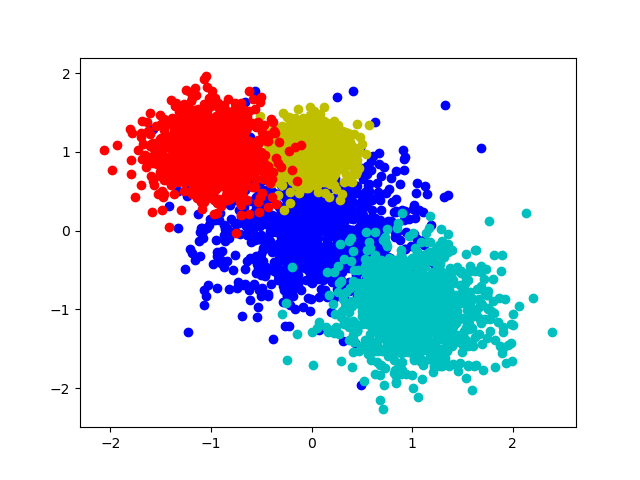
\includegraphics[width = .7\textwidth]{multi4.png}
   \label{dataset}
 \end{figure}
\end{frame}


\begin{frame}
  
    Explored SBM, BM, LBFGS, GD and SGD whose parameter settings are tuned and shown in table $\ref{parameter}$
    \begin{table}[htbp]
      \caption{parameter setting}
      \label{parameter}
      \centering
      \begin{tabular}{lllll}
        \toprule
        \multicolumn{5}{c}{$p:$ batch size $\quad$  $m:$ number of vectors in LBFGS }                   \\
        \cmidrule(r){1-5}
        BM     & SBM    & LBFGS & GD & SGD \\
        \midrule
        $\lambda = 1e-2$ &  $p = 40$  & $\eta:$ line search &$\lambda = 1e-2$ &$p = 40$      \\
         $\epsilon = 1e-6$    &  $\epsilon = 1e-6$  &  $\epsilon = 1e-5$ & $\epsilon = 1e-5$& $\epsilon = 1e-5$ \\
        $ \eta = 1$   &  $ \eta = 1e-2$   &  $m = 4$ &$\eta = 1e-2$ &$\eta = 1e-2$  \\
        \bottomrule
      \end{tabular}
    \end{table}

\end{frame}


\begin{frame}
\begin{block}{}
  \begin{figure}[htbp]
    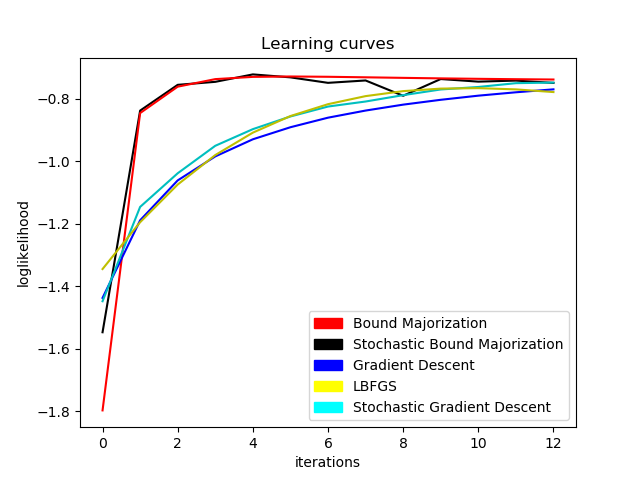
\includegraphics[width = .85\textwidth]{iterations}
    \caption{iteration comparison}
  \end{figure}
\end{block}
\end{frame}

\begin{frame}
  \begin{block}{}
    \begin{figure}[htbp]
      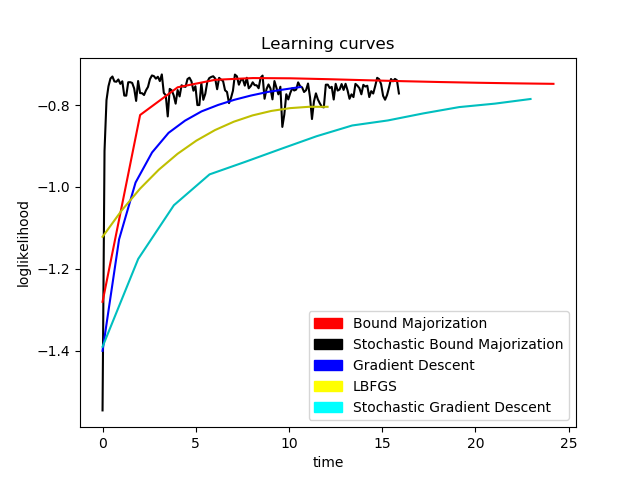
\includegraphics[width = .85\textwidth]{time}
      \caption{time comparison}
    \end{figure}
  \end{block}
  \end{frame}

  \begin{frame}
    \begin{block}{}
      \begin{figure}[htbp]
        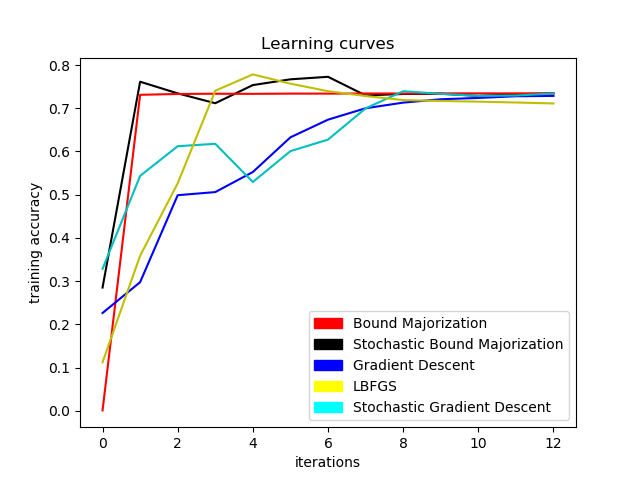
\includegraphics[width = .85\textwidth]{train_accuracy}
        \caption{training accuracy comparison}
      \end{figure}
    \end{block}
    \end{frame}

    \begin{frame}
      \begin{block}{}
        \begin{figure}[htbp]
          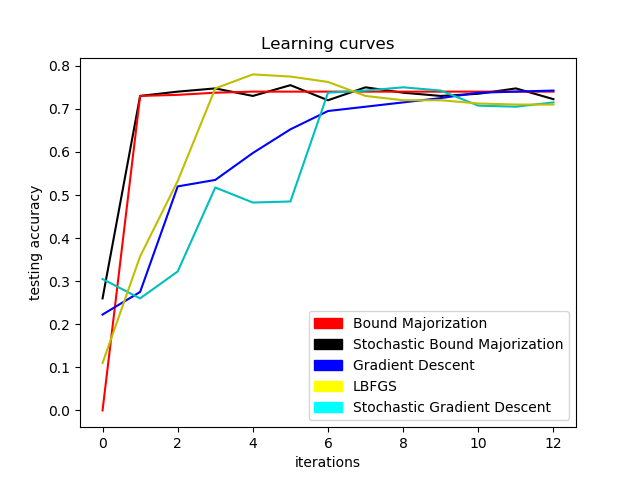
\includegraphics[width = .85\textwidth]{test_accuracy}
          \caption{testing accuracy comparison}
        \end{figure}
      \end{block}
      \end{frame}

\section{conclusion}

 \begin{frame}
  \begin{block}{Conclusion}
        \begin{itemize}
          \item Requiring very few parameters tuning, (stepsize $\eta$ or convex hull $\Lambda$);
       
          \item Bound is very tight, which makes it extremely efficient;
         
          \item Only applicable to log-linear models, CRFs, Latent Likelihoods etc.
          
          \item The assumptions and conditions has to be satisfied properly, otherwise it may diverge.
      
        \end{itemize}
      \end{block}
      \end{frame}

\begin{frame}
  \begin{block}{}
    \begin{equation}
      \mathbf{Thank} \ \mathbf{You} \mathbf{!} \nonumber
    \end{equation}
  \end{block}
\end{frame}


\end{document}
